\documentclass{article}
\usepackage{../assignment_preamble}

\title{Homework 4}
\author{Ravi Kini}
\date{December 12, 2025}

\begin{document}

\maketitle

\problem{}
\subproblem{(a)}
Let $L_n$ be the degree $n$ Legendre polynomial and $p(x)$ be some polynomial with degree less than $n$. W can represent $p(x) = \sum_{k=0}^{n-1} a_k x^k$. Then:
\begin{align*}
    \int_{-1}^1 L_n(x)p(x) \, dx & = \int_{-1}^1 L_n(x)\left(\sum_{k=0}^{n-1} a_k x^k\right) \, dx \\
    & = \sum_{k=0}^{n-1} a_k\int_{-1}^1 L_n(x)x^k \, dx
\end{align*}
To show that $\int_{-1}^1 L_n(x)p(x) \, dx = 0$, it is then sufficient to show that $\int_{-1}^1 L_n(x)x^k \, dx = 0$ for all $k < n$. Using Rodrigue' formula:
\begin{align*}
    \int_{-1}^1 L_n(x)x^k \, dx & = \int_{-1}^1 \left(\frac{1}{2^n n!}\frac{d^n}{dx^n} {(x^2 - 1)}^n\right) x^k \, dx \\
    & = \frac{1}{2^n n!}\int_{-1}^1 \left(\frac{d^n}{dx^n} {(x^2 - 1)}^n\right) x^k \, dx
\end{align*}
Applying integration by parts once:
\begin{align*}
    \int_{-1}^1 \left(\frac{d^n}{dx^n} {(x^2 - 1)}^n\right) x^k \, dx & = \left.\left(\frac{d^{n-1}}{dx^{n-1}} {(x^2 - 1)}^n\right) x^k \, dx \right\vert_{-1}^1 - \int_{-1}^1 \left(\frac{d^{n-1}}{dx^{n-1}} {(x^2 - 1)}^n\right) kx^{k-1} \, dx \\
    & = -\int_{-1}^1 \left(\frac{d^{n-1}}{dx^{n-1}} {(x^2 - 1)}^n\right) kx^{k-1} \, dx
\end{align*}
Clearly by qpplying integration by parts $n$ times, we get:
\begin{align*}
    \int_{-1}^1 \left(\frac{d^n}{dx^n} {(x^2 - 1)}^n\right) x^k \, dx & = \frac{{(-1)}^n k!}\int_{-1}^1 {(x^2 - 1)}^n \left(\frac{d^n}{dx^n}x^k\right) \, dx
\end{align*}
Since $k < n$, $\frac{d^n}{dx^n}x^k = 0$. It then follows that $\int_{-1}^1 L_n(x)x^k \, dx = 0$ for all $k < n$, and so $\int_{-1}^1 L_n(x)p(x) \, dx$ for an arbirary $p(x)$ with degree $k < n$.
\subproblem{(b)}
Let $\tilde{L}_n$ be the monic degree $n$ Legendre polynomial and $\tilde{p}(x)$ be some monic polynomial with degree $n$. Their difference $r(x) = \tilde{p}(x) - \tilde{L}_n(x)$ then has degree $k < n$. Since Legendre polynomial are orthogonal to polynomials of smaller degree:
\begin{align*}
    \langle \tilde{L}_n, r\rangle & = \int_{-1}^1 \tilde{L}_n(x)r(x) \, dx = 0
\end{align*}
Now, using the properties of the norm:
\begin{align*}
    ||tilde{p}||_2^2 & = \langle \tilde{p}, \tilde{p}\rangle \\
    & = \langle\tilde{L}_n + r, \tilde{L}_n + r\rangle \\
    & = \langle\tilde{L}_n, \tilde{L}_n\rangle + 2\langle\tilde{L}_n, r\rangle + \langle r, r\rangle \\
    & = \langle\tilde{L}_n, \tilde{L}_n\rangle + \langle r, r\rangle \\
    & = ||\tilde{L}_n||_2^2 + ||r||_2^2
\end{align*}
Since $||r||_2^2 \geq 0$, $|tilde{p}||_2^2 \geq ||\tilde{L}_n||_2^2$ for all such $\tilde{p}$.

\clearpage
\problem{}
\subproblem{(a)}
Let $p(x) = 2^{-n}(T_{n+1}(x) - T_{n-1}(x))$, where $T_n(x)$ is the $n$th degree Chebyshev polynomial. Then, letting $x_k = \cos(k\pi/n)$ for $k \in \{0, \ldots, n\}$:
\begin{align*}
    p(x_k) & = 2^{-n}(T_{n+1}(x_k) - T_{n-1}(x_k)) \\
    & = 2^{-n}(T_{n+1}(\cos(k\pi/n)) - T_{n-1}(\cos(k\pi/n))) \\
    & = 2^{-n}(\cos((n + 1)k\pi/n) - \cos((n - 1)k\pi/n)) \\
    & = 2^{-n}(\cos(k\pi + k\pi/n) - \cos(k\pi - k\pi/n))
\end{align*}
If $k$ is even:
\begin{align*}
    p(x_k) & = 2^{-n}(\cos(k\pi/n) - \cos(- k\pi/n)) \\
    & = 2^{-n}(\cos(k\pi/n) - \cos(k\pi/n)) = 0
\end{align*}
If $k$ is odd:
\begin{align*}
    p(x_k) & = 2^{-n}(\cos(\pi + k\pi/n) - \cos(\pi - k\pi/n)) \\
    & = 2^{-n}(-\cos(k\pi/n) + \cos(-k\pi/n)) \\
    & = 2^{-n}(-\cos(k\pi/n) + \cos(k\pi/n)) = 0
\end{align*}
In either case, $x_k$ is a root of $p(x)$ for all $k$. Note that $p(x)$ has degree $n + 1$ (since $T_{n+1}$ is of degree $n + 1$, and $T_{n-1}$ is of lesser degree), and so can have at most $n + 1$ roots, which must then be $x_0, \ldots, x_n$. For the same reason, $T_{n+1}(x) - T_{n-1}(x)$ has leading coefficient $2^n$, and so $p(x)$ has leading coefficient $2^{-n} \cdot 2^n = 1$, making it monic. $p(x)$ is then the unique monic polynomial with degree $n + 1$ and roots $x_0, \ldots, x_n$.
\subproblem{(b)}
\begin{lstlisting}[language=Python]
import numpy as np, scipy as sp
import matplotlib.pyplot as plt

def equally_spaced(n):
  return np.array([-1 + 2 * k / n for k in range(n + 1)])

def extrema(n):
  return np.array([np.cos(k * np.pi / n) for k in range(n + 1)])

def zeros(n):
  return np.array([np.cos((2 * k - 1) * np.pi / (2 * (n + 1))) for k in range(1, n + 2)])

def interpolate(f, n, typ):
  if typ == 'equally spaced':
      x = equally_spaced(n)
  if typ == 'extrema':
      x = extrema(n)
  if typ == 'zeros':
      x = zeros(n)
  y = f(x)
  return sp.interpolate.lagrange(x, y)
\end{lstlisting}
The following table shows the maximum approximation error when using $n$ equally spaced points to interpolate the functions $f_1(x) = \mathrm{exp}(-(x - 0.5)^2)$, $f_2(x) = {(16x^2 + 1)}^{-1}$, and $f_3(x) = x|x|$ on the interval $[-1, 1]$:
\begin{center}
\begin{tabular}{|c|c|c|c|}
    \hline
    $n$ & $f_1$ & $f_2$ & $f_3$ \\ 
    \hline
    $4$ & $1.911 \cdot 10^{-2}$ & $3.853 \cdot 10^{-1}$ & $3.208 \cdot 10^{-2}$ \\
    \hline
    $8$ & $2.224 \cdot 10^{-4}$ & $7.319 \cdot 10^{-1}$ & $1.439 \cdot 10^{-2}$ \\
    \hline
    $12$ & $1.099 \cdot 10^{-6}$ & $1.969 \cdot 10^0$ & $2.867 \cdot 10^{-2}$ \\
    \hline
    $16$ & $6.835 \cdot 10^{-9}$ & $5.911 \cdot 10^0$ & $1.071 \cdot 10^{-1}$ \\
    \hline
    $20$ & $12.382 \cdot 10^{-6}$ & $1.875 \cdot 10^1$ & $5.630 \cdot 10^{-1}$ \\
    \hline
\end{tabular}
\end{center}
Instead using the extrema of $T_n$:
\begin{center}
\begin{tabular}{|c|c|c|c|}
    \hline
    $n$ & $f_1$ & $f_2$ & $f_3$ \\ 
    \hline
    $4$ & $2.067 \cdot 10^{-2}$ & $3.708 \cdot 10^{-1}$ & $5.047 \cdot 10^{-2}$ \\
    \hline
    $8$ & $7.735 \cdot 10^{-5}$ & $1.307 \cdot 10^{-1}$ & $1.198 \cdot 10^{-2}$ \\
    \hline
    $12$ & $9.586 \cdot 10^{-8}$ & $4.251 \cdot 10^{-2}$ & $5.271 \cdot 10^{-3}$ \\
    \hline
    $16$ & $2.068 \cdot 10^{-10}$ & $1.754 \cdot 10^{-2}$ & $2.955 \cdot 10^{-3}$ \\
    \hline
    $20$ & $3.614 \cdot 10^{-8}$ & $6.671 \cdot 10^{-3}$ & $1.888 \cdot 10^{-3}$ \\
    \hline
\end{tabular}
\end{center}
Instead using the positive zeros of $T_{n + 1}$:
\begin{center}
\begin{tabular}{|c|c|c|c|}
    \hline
    $n$ & $f_1$ & $f_2$ & $f_3$ \\ 
    \hline
    $4$ & $1.199 \cdot 10^{-2}$ & $3.118 \cdot 10^{-1}$ & $3.858 \cdot 10^{-2}$ \\
    \hline
    $8$ & $4.361 \cdot 10^{-5}$ & $1.039 \cdot 10^{-1}$ & $9.995 \cdot 10^{-3}$ \\
    \hline
    $12$ & $6.225 \cdot 10^{-8}$ & $3.789 \cdot 10^{-2}$ & $4.611 \cdot 10^{-3}$ \\
    \hline
    $16$ & $1.068 \cdot 10^{-9}$ & $1.484 \cdot 10^{-2}$ & $2.658 \cdot 10^{-3}$ \\
    \hline
    $20$ & $1.785 \cdot 10^{-7}$ & $5.498 \cdot 10^{-3}$ & $1.730 \cdot 10^{-3}$ \\
    \hline
\end{tabular}
\end{center}
Plotting the approximation error for $f_1$, with $n = 8$ and $n = 20$:
\begin{center}
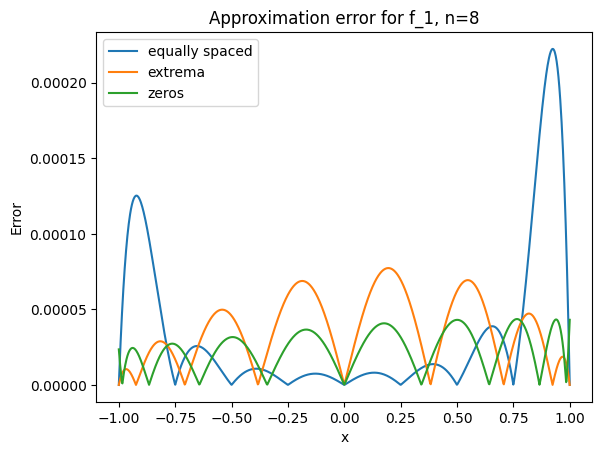
\includegraphics[width=0.45\textwidth]{../../img/mat226a/hw4/2b_f1_8.png}
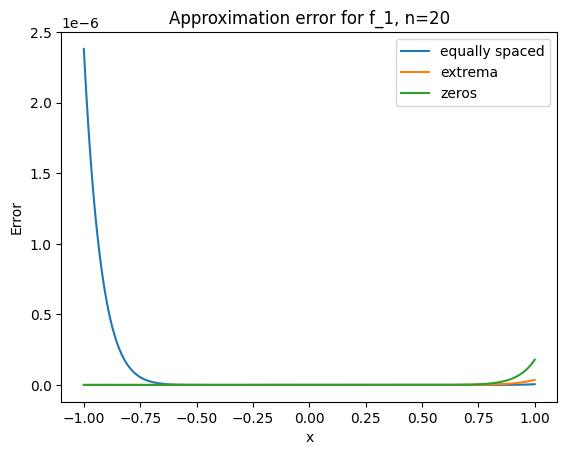
\includegraphics[width=0.45\textwidth]{../../img/mat226a/hw4/2b_f1_20.png}
\end{center}
For $f_2$:
\begin{center}
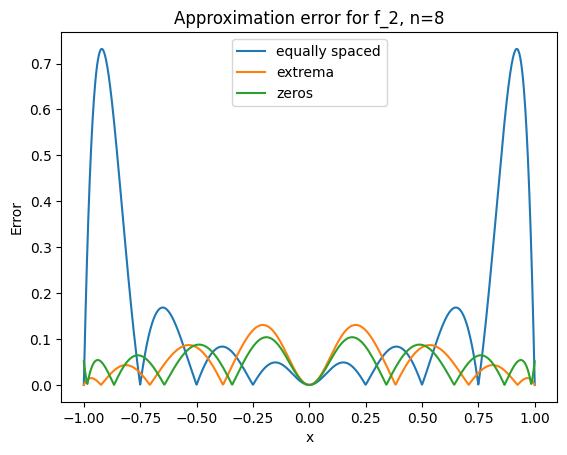
\includegraphics[width=0.45\textwidth]{../../img/mat226a/hw4/2b_f2_8.png}
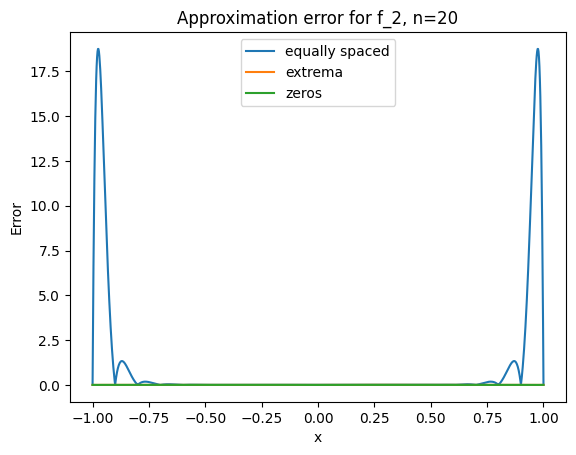
\includegraphics[width=0.45\textwidth]{../../img/mat226a/hw4/2b_f2_20.png}
\end{center}
For $f_3$:
\begin{center}
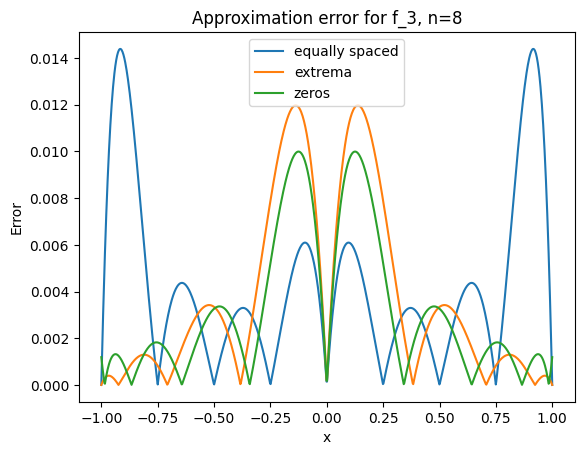
\includegraphics[width=0.45\textwidth]{../../img/mat226a/hw4/2b_f3_8.png}
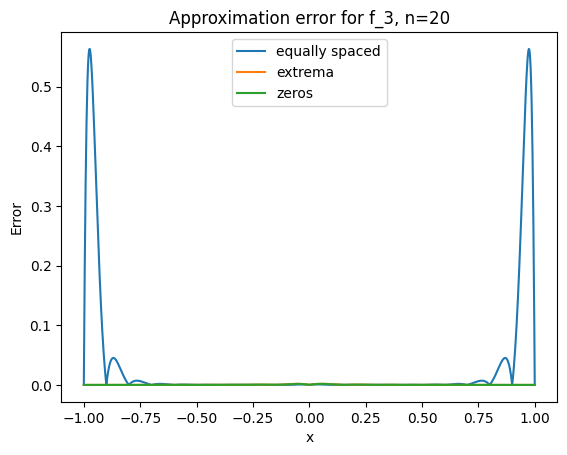
\includegraphics[width=0.45\textwidth]{../../img/mat226a/hw4/2b_f3_20.png}
\end{center}

For $f_1$ and $f_3$, all three methods perform comparably, likely because $f_1'(x) = -2(x - 0.5)\mathrm{exp}(-(x - 0.5)^2)$ and $f_3'(x) = 2x\mathrm{sign}(x)$ do not change very rapidly. For $f_2$, using qually spaced points has a much higher maximum approximation error than the other two methods, likely, because $f_2'(x) = -32x(16x^2 + 1)^{-2}$ changes much more rapidly, particularly as it crosses $x = 0$.

\subproblem{(c)}
Comparing the two types of Chebyshev points used, they produce comparable maximum approximation errors. From the result derived in part (a), since $p(x)$ is the unique monic polynomial with roots at $x_k$, which are also the extrema of $T_n$, using those as the interpolation points minimizes the maximum approximation error.

\clearpage
\problem{}
\begin{lstlisting}[language=Python,breaklines=True]
import numpy as np
import matplotlib.pyplot as plt

def composite_trapezoidal(f, a, b, n):
  h = (b - a) / n
  x = np.linspace(a, b, n + 1)
  y = f(x)
  return h * (0.5 * y[0] + np.sum(y[1:-1]) + 0.5 * y[-1])

def composite_simpsons(f, a, b, n):
  h = (b - a) / n
  x = np.linspace(a, b, n + 1)
  y = f(x)
  return h / 3 * (y[0] + 4 * np.sum(y[1:-1:2]) + 2 * np.sum(y[2:-1:2]) + y[-1])

def composite_3pt_gaussian_quad(f, a, b, n):
  n = np.array([-np.sqrt(3/5), 0, np.sqrt(3/5)])
  w = np.array([5/9, 8/9, 5/9])
  h = (b - a) / n
  integral = 0.0
  for i in range(n):
      xl, xr = a + i * h, a + (i + 1) * h
      xm, xh = (xl + xr) / 2, (xr - xl) / 2
      y =  f(xm + xh * n)
      integral += xh * np.sum(w * y)
  return integral

def composite_4pt_gaussian_quad(f, a, b, n):
  n = np.array([-np.sqrt((3 + 2*np.sqrt(6/5)) / 7), -np.sqrt((3 - 2*np.sqrt(6/5)) / 7), np.sqrt((3 - 2*np.sqrt(6/5)) / 7), np.sqrt((3 + 2*np.sqrt(6/5)) / 7)])
  w = np.array([(18 - np.sqrt(30)) / 36, (18 + np.sqrt(30)) / 36, (18 + np.sqrt(30)) / 36, (18 - np.sqrt(30)) / 36])
  h = (b - a) / n
  integral = 0.0
  for i in range(n):
      xl, xr = a + i * h, a + (i + 1) * h
      xm, xh = (xl + xr) / 2, (xr - xl) / 2
      y =  f(xm + xh * n)
      integral += xh * np.sum(w * y)
  return integral
\end{lstlisting}
The composite trapezoidal rule and composite Simpson's rule require $n + 1$ function evaluations. Composite 3-point Gaussian quadrature and composite 4-point Gaussian quadrature require $3n$ and $4n$ function evaluations, respectively.

\subproblem{(b)}
The following table shows the results of approximating $\int_0^1 x \mathrm{exp}(-8x^2) \, dx$ using the four methods:
\begin{center}
\begin{tabular}{|c|c|c|c|c|}
    \hline
    $n$ & trapezoidal & Simpon's & 3 point & 4 point \\ 
    \hline
    $2$ & $3.392 \cdot 10^{-2}$ & $4.517 \cdot 10^{-2}$ & $6.254 \cdot 10^{-2}$ & $6.248 \cdot 10^{-2}$ \\
    \hline
    $4$ & $5.695 \cdot 10^{-2}$ & $6.463 \cdot 10^{-2}$ & $6.248 \cdot 10^{-2}$ & $6.248 \cdot 10^{-2}$ \\
    \hline
    $8$ & $6.115 \cdot 10^{-2}$ & $6.256 \cdot 10^{-2}$ & $6.248 \cdot 10^{-2}$ & $6.248 \cdot 10^{-2}$ \\
    \hline
    $16$ & $6.215 \cdot 10^{-2}$ & $6.248 \cdot 10^{-2}$ & $6.248 \cdot 10^{-2}$ & $6.248 \cdot 10^{-2}$ \\
    \hline
    $32$ & $6.240 \cdot 10^{-2}$ & $6.248 \cdot 10^{-2}$ & $6.248 \cdot 10^{-2}$ & $6.248 \cdot 10^{-2}$ \\
    \hline
\end{tabular}
\end{center}
and the following table shows the errors when compared with the actual result of $(1 - e^{-8})/16$:
\begin{center}
\begin{tabular}{|c|c|c|c|c|}
    \hline
    $n$ & trapezoidal & Simpon's & 3 point & 4 point \\ 
    \hline
    $2$ & $2.856 \cdot 10^{-2}$ & $1.731 \cdot 10^{-2}$ & $6.042 \cdot 10^{-5}$ & $-8.620 \cdot 10^{-7}$ \\
    \hline
    $4$ & $5.529 \cdot 10^{-3}$ & $2.148 \cdot 10^{-3}$ & $6.251 \cdot 10^{-7}$ & $-5.434 \cdot 10^{-9}$ \\
    \hline
    $8$ & $1.325 \cdot 10^{-3}$ & $7.619 \cdot 10^{-5}$ & $7.886 \cdot 10^{-9}$ & $-1.573 \cdot 10^{-11}$ \\
    \hline
    $16$ & $3.282 \cdot 10^{-4}$ & $4.157 \cdot 10^{-6}$ & $1.177 \cdot 10^{-10}$ & $-5.779 \cdot 10^{-14}$ \\
    \hline
    $32$ & $8.185 \cdot 10^{-5}$ & $2.521 \cdot 10^{-7}$ & $1.819 \cdot 10^{-12}$ & $-2.151 \cdot 10^{-16}$ \\
    \hline
\end{tabular}
\end{center}
Plotting the error in the approximation against the number of function evaluations for each of the methods:
\begin{center}
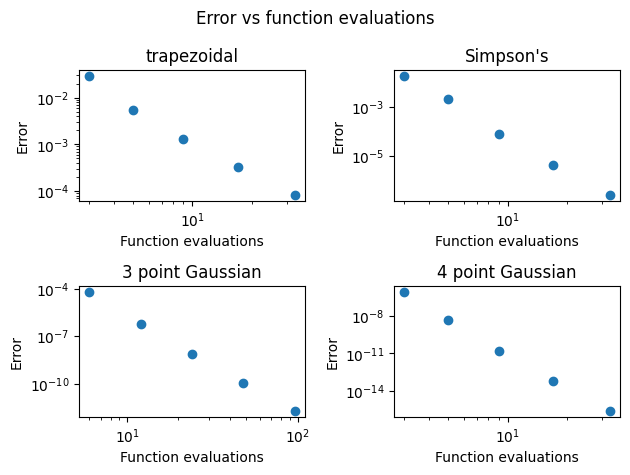
\includegraphics[width=0.7\textwidth]{../../img/mat226a/hw4/3b.png}
\end{center}
We see that the composite trapezoidal method converges at a rate of approximately $O(n^{2.4})$, composite Simpson's at a rate of approximately $O(n^{4.7})$, 3 point Gaussian quadrature at a rate of appximately $O(n^{6.2})$, and 4 point Gaussian quadrature at a rate of appximately $O(n^{9.2})$. Evidently, 4 point Gaussian quadrature converges the fastest, and trapezoidal the slowest, with the both requiring a number of function evaluations that is linear in $n$.

\subproblem{(c)}
The following table shows the results of approximating $\int_0^1 \sqrt{x} \, dx$ using the four methods:
\begin{center}
\begin{tabular}{|c|c|c|c|c|}
    \hline
    $n$ & trapezoidal & Simpon's & 3 point & 4 point \\ 
    \hline
    $2$ & $6.036 \cdot 10^{-1}$ & $6.381 \cdot 10^{-1}$ & $6.676 \cdot 10^{-1}$ & $6.671 \cdot 10^{-1}$ \\
    \hline
    $4$ & $6.433 \cdot 10^{-1}$ & $6.565 \cdot 10^{-1}$ & $6.670 \cdot 10^{-1}$ & $6.668 \cdot 10^{-1}$ \\
    \hline
    $8$ & $6.581 \cdot 10^{-1}$ & $6.631 \cdot 10^{-1}$ & $6.668 \cdot 10^{-1}$ & $6.667 \cdot 10^{-1}$ \\
    \hline
    $16$ & $6.636 \cdot 10^{-1}$ & $6.654 \cdot 10^{-1}$ & $6.667 \cdot 10^{-1}$ & $6.667 \cdot 10^{-1}$ \\
    \hline
    $32$ & $6.656 \cdot 10^{-1}$ & $6.662 \cdot 10^{-1}$ & $6.667 \cdot 10^{-1}$ & $6.667 \cdot 10^{-1}$ \\
    \hline
\end{tabular}
\end{center}
and the following table shows the errors when compared with the actual result of $2/3$:
\begin{center}
\begin{tabular}{|c|c|c|c|c|}
    \hline
    $n$ & trapezoidal & Simpon's & 3 point & 4 point \\ 
    \hline
    $2$ & $6.311 \cdot 10^{-2}$ & $2.860 \cdot 10^{-2}$ & $8.888 \cdot 10^{-4}$ & $4.105 \cdot 10^{-4}$ \\
    \hline
    $4$ & $2.338 \cdot 10^{-2}$ & $1.014 \cdot 10^{-2}$ & $3.142 \cdot 10^{-4}$ & $1.451 \cdot 10^{-4}$ \\
    \hline
    $8$ & $8.536 \cdot 10^{-3}$ & $3.587 \cdot 10^{-3}$ & $1.111 \cdot 10^{-4}$ & $5.131 \cdot 10^{-5}$ \\
    \hline
    $16$ & $3.085 \cdot 10^{-3}$ & $1.268 \cdot 10^{-3}$ & $3.928 \cdot 10^{-5}$ & $1.814 \cdot 10^{-5}$ \\
    \hline
    $32$ & $1.108 \cdot 10^{-3}$ & $4.485 \cdot 10^{-4}$ & $1.389 \cdot 10^{-5}$ & $6.414 \cdot 10^{-6}$ \\
    \hline
\end{tabular}
\end{center}
Plotting the error in the approximation against the number of function evaluations for each of the methods:
\begin{center}
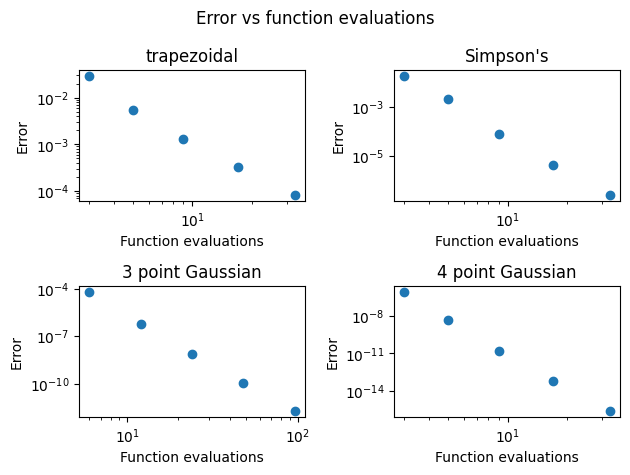
\includegraphics[width=0.7\textwidth]{../../img/mat226a/hw4/3b.png}
\end{center}
We see that the composite trapezoidal method converges at a rate of approximately $O(n^{1.7})$, composite Simpson's at a rate of approximately $O(n^{1.7})$, 3 point Gaussian quadrature at a rate of appximately $O(n^{1.5})$, and 4 point Gaussian quadrature at a rate of appximately $O(n^{1.7})$. All four methods converge sloswer for this problem, notably with 3 point Gaussian quadrature converging the slowest. This is likely because this function is not smooth, as its derivative is singular at $x = 0$.

\clearpage
\problem{}
\subproblem{(a)}
\begin{lstlisting}
import numpy as np

func_eval = 0

def simps(a, b, fa, fm, fb):
  h = (b - a) / 2
  return h / 3 * (fa + 4 * fm + fb)

def adapt(f, a, b, sab, fa, fab2, fb, tol, nodes):
  global func_eval
  xab2 = (a + b) / 2
  xm1, xm2 = (3 * a + b) / 4, (a + 3 * b) / 4
  fm1, fm2 = f(xm1), f(xm2)
  func_eval += 2
  new_nodes = nodes + [xm1, xm2]
  sm1, sm2 = simps(a, xab2, fa, fm1, fab2), simps(xab2, b, fab2, fm2, fb)
  factor = 15
  if abs(sm1 + sm2 - sab) < factor * tol:
    q = sm1 + sm2
  else:
    q1, new_nodes = adapt(f, a, xab2, sm1, fa, fm1, fab2, tol / 2, new_nodes)
    q2, new_nodes = adapt(f, xab2, b, sm2, fab2, fm2, fb, tol / 2, new_nodes)
    q = q1 + q2
  return q, new_nodes

def adaptive_simpson(f, a, b, tol):
  global func_eval
  fa, fab2, fb = f(a), f((a + b) / 2), f(b)
  func_eval += 3
  sab = simps(a, b, fa, fab2, fb)
  nodes = [a, (a + b) / 2, b]
  q, new_nodes = adapt(f, a, b, sab, fa, fab2, fb, tol, nodes)
  return q, new_nodes, func_eval
\end{lstlisting}
The following table shows the errors of approximating $\int_0^1 \frac{1}{x + 0.001} \, dx$ using adaptive Simpson's quadrature when compared with the actual result of $\ln 1001$:
\begin{center}
\begin{tabular}{|c|c|c|c|c|}
    \hline
    Tolerance & $10^{-4}$ & $10^{-6}$ & $10^{-8}$ & $10^{-10}$ \\
    \hline
    Error & $2.527 \cdot 10^{-5}$ & $3.734 \cdot 10^{-7}$ & $3.341 \cdot 10^{-9}$ & $3.519 \cdot 10^{-11}$ \\
    \hline
    Function evaluations & $161$ & $509$ & $1617$ & $5057$ \\
    \hline
\end{tabular}
\end{center}
As the tolerance decreases, the number of required function evaluatiosn grows. Checking the set of points at which the function was evaluated, several of the points are close to $x = 0$; this is because the derivative of the integrand is large in this region.
\subproblem{(b)}
Let $h = 1/n$ and $x_k = (k - 1)/h$. We then define $g_k(t)$ such that:
\begin{align*}
    g_k(t) = \frac{t}{2}(f(x_k) + f(x_k + t)) - \int_{x_k}^{x_k + t} f(x) \, dx
\end{align*} 
We see that $g_k(h)$ is the error of the trapezoidal rule on the interval $[x_k, x_k + h]$. Then:
\begin{align*}
    \frac{dg_k}{dt} & = \frac{1}{2}(f(x_k) + f(x_k + t)) + \frac{t}{2}f'(x_k + t) - f(x_k + t) \\
    \frac{d^2g_k}{dt^2} & = \frac{t}{2}f''(x_k + t)
\end{align*}
Let $\xi \in [0, 1]$ such that $f''(\xi)$ is maximum. Since the function is sufficiently smooth, $|f''(x)| \leq |f''(\xi)|$ for all $x \in [0, 1]$, and so $|f''(x_k + t)| \leq |f''(\xi)|$. Then, since $g'_k(0), g_k(0) = 0$:
\begin{align*}
    \int_0^t g''_k(t') \, dt' & = g'_k(t) \\
    \int_0^t g'_k(t') \, dt' & = g_k(t) \\
\end{align*}
It follows, integrating over $t$ that:
\begin{align*}
    -\frac{t}{2}f''(\xi) & \leq g''_k(t) \leq \frac{t}{2}f''(\xi) \\
    -\frac{t^2}{4}f''(\xi) & \leq g'_k(t) \leq \frac{t^2}{4}f''(\xi) \\
    -\frac{t^3}{12}f''(\xi) & \leq g_k(t) \leq \frac{t^3}{12}f''(\xi) \\
    -\frac{h^3}{12}f''(\xi) & \leq g_k(h) \leq \frac{h^3}{12}f''(\xi)
\end{align*}
Summing over the error terms for all of the intervals:
\begin{align*}
    -\sum_{k=1}^n \frac{h^3}{12}f''(\xi) & \leq \sum_{k=1}^n g_k(h) \leq \sum_{k=1}^n \frac{h^3}{12}f''(\xi) \\
    -n\frac{h^3}{12}f''(\xi) & \leq \sum_{k=1}^n g_k(h) \leq n\frac{h^3}{12}f''(\xi) \\
    \left|\sum_{k=1}^n g_k(h)\right| & \leq \frac{1}{12n^2}|f''(\xi)|
\end{align*}
If $f(x) = \frac{1}{x + 0.001}$, $f''(x) = \frac{2}{(x + 0.001)^3}$, which is maximum at $\xi = 0$, where $f''(\xi) = 2 \cdot 10^9$. We then see that the error is bounded by:
\begin{align*}
    \textrm{err} \leq \frac{1}{6n^2} \cdot 10^9
\end{align*}
To guarantee that the error is below $10^{-10}$ using the composite trapezoidal rule, it follows that the number of points required is upper bounded by $\sqrt{10^{19}/6} \approx 1.29 \cdot 10^9$.

We now instead define $g_k(t)$ such that:
\begin{align*}
    g_k(t) = \frac{t}{3}(f(x_k - t) + 4f(x_k) + f(x_k + t)) - \int_{x_k - t}^{x_k + t} f(x) \, dx
\end{align*} 
We see that $g_k(h/2)$ is the error of Simpson's rule on the interval $[x_k - h/2, x_k + h/2]$. Then:
\begin{align*}
    \frac{dg_k}{dt} & = \frac{1}{3}(-2f(x_k - t) + 4f(x_k) - 2f(x_k + t)) - \frac{t}{3}(f'(x_k - t) - f'(x_k + t)) \\
    \frac{d^2g_k}{dt^2} & = \frac{1}{3}(f'(x_k - t) - f'(x_k + t)) + \frac{t}{3}(f''(x_k - t) + f''(x_k + t)) \\
    \frac{d^3g_k}{dt^3} & = -\frac{t}{3}(f^{(3)}(x_k + t) - f^{(3)}(x_k - t))
\end{align*}
Let $\xi \in [0, 1]$ such that $f^{(4)}(\xi)$ is maximum. Since the function is sufficiently smooth, $|f^{(4)}(x)| \leq |f^{(4)}(\xi)|$ for all $x \in [0, 1]$, and so $|f^{(4)}(x_k + t)| \leq |f^{(4)}(\xi)|$. Then, since $g''_k(0), g'_k(0), g_k(0) = 0$, applying the extended mean theorem, for some $t'$, $t''$:
\begin{align*}
    \frac{g_k(t)}{t^5} & = \frac{g^{(3)}(t')}{60{t'}^2} \\
    & = -\frac{1}{90t'}(f^{(3)}(x_k + t') - f^{(3)}(x_k - t')) \\
    & = -\frac{1}{90}f^{(4)}(t'')
\end{align*}
Then:
\begin{align*}
    |g_k(t)| & \leq \left|\frac{t^5}{90}f^{(4)}(\xi)\right| \\
    |g_k(h)| & \leq \left|\frac{h^5}{90}f^{(4)}(\xi)\right|
\end{align*}
Summing over the error terms for all of the intervals:
\begin{align*}
    \left|\sum_{k=1}^n g_k(h) \right| \leq \sum_{k=1}^n |g_k(h)| & \leq \sum_{k=1}^n \left|\frac{h^5}{90}f^{(4)}(\xi)\right| \\
    & \leq n\left|\frac{h^5}{90}f^{(4)}(\xi)\right| \\
    & \leq \frac{1}{90n^5}\left|f^{(4)}(\xi)\right|
\end{align*}
If $f(x) = \frac{1}{x + 0.001}$, $f^{(4)}(x) = \frac{24}{(x + 0.001)^5}$, which is maximum at $\xi = 0$, where $f''(\xi) = 2 \cdot 10^{15}$. We then see that the error is bounded by:
\begin{align*}
    \textrm{err} \leq \frac{4}{15n^5} \cdot 10^{15}
\end{align*}
To guarantee that the error is below $10^{-10}$ using the composite Simpson's rule, it follows that the number of points required is upper bounded by $\sqrt[5]{4 \cdot 10^{25}/15} \approx 76770$.

\subproblem{(c)}
\begin{lstlisting}[language=Python]
err = 100
n = 1
while err > 1e-10:
  res = composite_simpsons(f, 0, 1, n)
  err = abs(res - np.log(1001))
  n += 1
print(res, err, n)
\end{lstlisting}
In reality, only 5057 points are rquired to get the error below $10^{-10}$. This is much lower than the analytic bound, which is likely a product of the high values of the derivatives around $\xi = 0$ to get a precise approximation close to this point.
\end{document}